\documentclass[10pt, notes]{beamer}

\input{lib.tex}
\usepackage{comment}
\usepackage{pgfpages}
\usepackage{bm}


\usetheme[progressbar=frametitle]{metropolis}
\tikzset{font={\fontsize{10pt}{12}\selectfont}}
\usepackage{hf-tikz}
\usetikzlibrary{ 
	calc,
	arrows,
	arrows.meta,
	automata, 
	shapes, 
	snakes, 
	positioning, 
	decorations,
	decorations.text,
	fit,
	matrix,
	mindmap
	}
	\tikzstyle{noeud-std}=[draw,fill=black,circle,inner sep=0pt,minimum size=7pt]% 7pt est la taille des cercles noirs
\usepackage{tkz-graph}
\newcommand{\tikzmark}[2]{\tikz[overlay,remember picture,baseline=(#1.base)] \node (#1) {#2};}
\newcommand{\Highlight}[1][submatrix]{%
    \tikz[overlay,remember picture]{
    \node[highlight,fit=(left.north west) (right.south east)] (#1) {};}
    }
\tikzset{%
  highlight/.style={rectangle,rounded corners,fill=ocre!50,draw,
    fill opacity=0.5,thick,inner sep=0pt}
}
\newcommand{\mytikzmark}[2]{\tikz[overlay,remember picture, baseline=(#1.base)] \node (#1) {#2};}

\usepackage{xspace}
\usepackage{amsmath}
\usepackage{mathtools}

\usepackage[doi=false,isbn=false,note=false,url=false,eprint=false, backend=bibtex]{biblatex} 
\AtEveryCitekey{\clearfield{note}\clearlist{location}\clearlist{publisher}\clearname{editor}}
\bibliographystyle{plain}
\bibliography{biblio}

\definecolor{green}{HTML}{14B03D}
\newcommand{\payoff}[2]{{\color{green}#1}, {\color{red}#2}}

\title{LINMA2345 - Game theory}
\subtitle{Repeated games}
\date{\today}
\author{Antoine Gennart\and Jonathan Sarteel\and Antoine Paris}
\institute{Ecole polytechnique de Louvain}
\titlegraphic{\hfill\includegraphics[height=1cm]{logo}}

\begin{document}
\maketitle

\begin{frame}{Outline}
    \setbeamertemplate{sections in toc}[sections numbered]
    \tableofcontents[hideallsubsections]
\end{frame}

\begin{frame}{Outline}
    \tableofcontents[currentsection]
\end{frame}

\section{Finitely repeated games}
\begin{frame}{What is a finitely repeated games?}
    In a \textit{finitely repeated game}, players
    \begin{itemize}
        \item play the same game for a finite number of times $K$,
        \textbf{known by the players before the game starts}, and
        \item collect their payoffs after each round (and thus observe what
        the others played).
    \end{itemize}

    \begin{figure}[!ht]
        \centering
        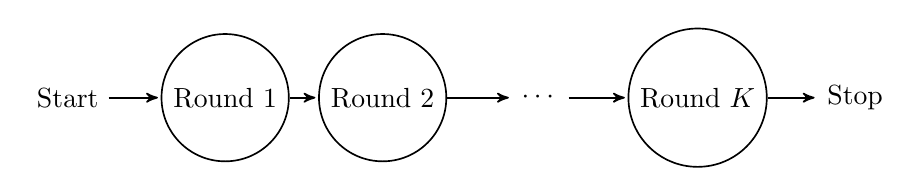
\begin{tikzpicture}[->,>=stealth',shorten >=1pt,auto,node distance=2cm, semithick, scale = 1,
            transform shape ]
            \node	        (start)								{Start};
            \node[state] 	(n1)    	[right of = start]		{Round 1};
            \node[state] 	(n2)		[right of = n1]			{Round 2};
            \node	        (dots)		[right of = n2]			{$\cdots$};
            \node[state] 	(nk)		[right of = dots]		{Round $K$};
            \node	        (stop)		[right of = nk]			{Stop};
            \path 	(start) edge node {}	(n1)
                    (n1)	edge node {}	(n2)
                    (n2)	edge node {}	(dots)
                    (dots)	edge node {}	(nk)
                    (nk) 	edge node {}	(stop);
        \end{tikzpicture}
        \caption{Finitely Repeated Games.}
    \end{figure}
\end{frame}

\begin{frame}{Let's play the Prisoner's Dilemma 2 times}
    \begin{exampleblock}{Example}
        Consider the Prisoner's Dilemma in normal form.
        \begin{table}
            \begin{tabular}{c|cc}
                & {\color{red}c}    & {\color{red}d} \\
                \hline
                {\color{green}C}    & \payoff{-1}{-1}   & \payoff{-4}{~0} \\
                {\color{green}D}    & \payoff{~0}{-4}    & \payoff{-3}{-3} 
            \end{tabular}
            \caption{Prisoner's Dilemma in normal form.}
        \end{table}
    
        \begin{itemize}
            \item The only Nash Equilibrium of this game is for both
            players to defect.
            \item Let's play this game 2 times in a row and see what happens.
        \end{itemize}
        
        \vspace{0.5cm}
        \hfill \textit{Hint}: \reflectbox{think backward}.

    \end{exampleblock}
\end{frame}

\note{
    Draw a table on the blackboard and collect the actions/outcomes of each pair
    of students after each round.

    At the end, quickly compare the result. Ask students to motivate their strategy
    choice (especially if it differs from what a rationnal player would do).

    Probably the audience will cooperate more than expected.
}

\begin{frame}{The twice repeated Prisoner's Dilemma: Nash Equilibrium}
We proceed by \textit{backward induction} to find the Nash Equilibrium.
\begin{figure}[!ht]
    \centering
    \scalebox{0.65}{
    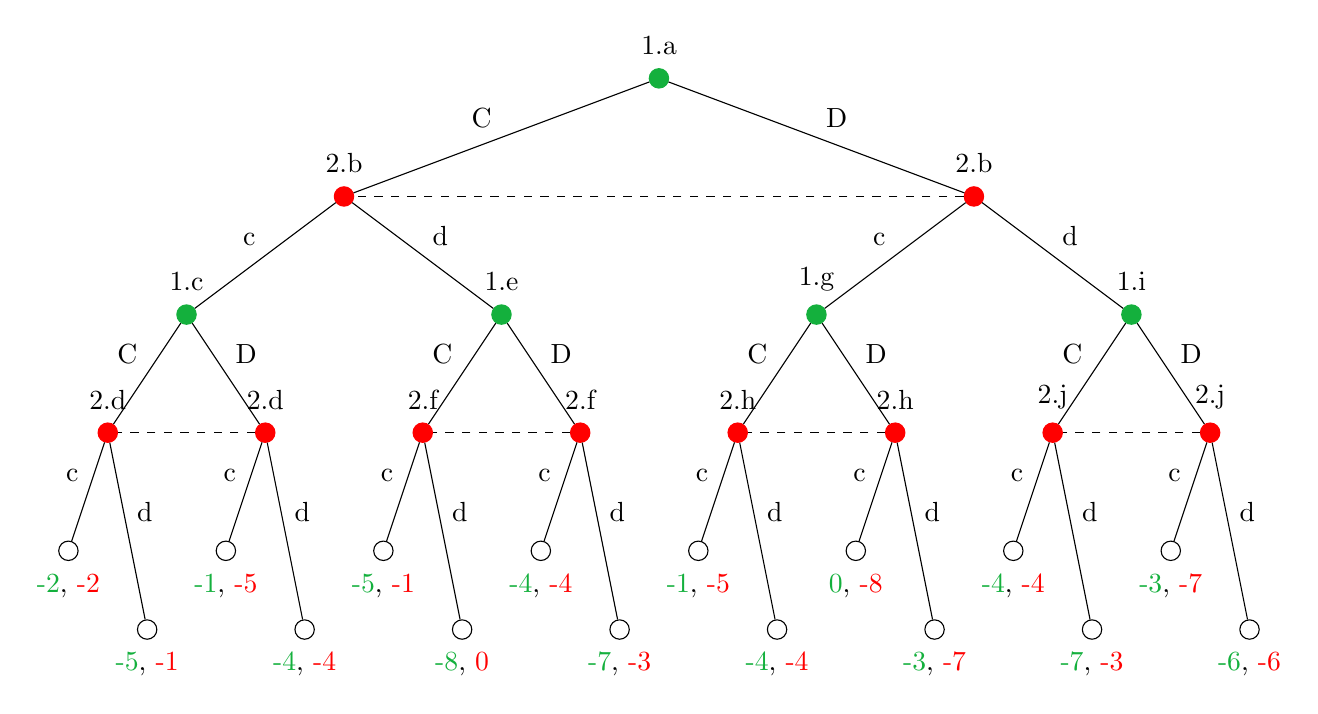
\begin{tikzpicture}
    \node[noeud-std, color=green] (n1) {}
       [sibling distance=8cm]
          child {node[noeud-std, color=red] (n2-1c) {} % 1
          [sibling distance=4cm]
                 child{node[noeud-std, color=green] (n1-1c2c){} % 2
                    [sibling distance=2cm]
                    child{node[noeud-std, color=red] (n2-1c2c1c){}  % 1
                        [sibling distance = 1cm]
                             child[level distance=1.5cm]{node[noeud-std,fill=white] (p-1c2c1c2c){} } % 1
                             child[level distance=2.5cm]{node[noeud-std,fill=white] (p-1c2c1c2d){} } % 1
                         }
                    child{node[noeud-std, color=red] (n2-1c2c1d){}  % 1
                        [sibling distance = 1cm]
                            child[level distance=1.5cm]{node[noeud-std,fill=white] (p-1c2c1d2c){} } % 1
                            child[level distance=2.5cm]{node[noeud-std,fill=white] (p-1c2c1d2d){} } % 1
                        }
                }
                child{node[noeud-std, color=green] (n1-1c2d){} % 2
                    [sibling distance=2cm]
                    child{node[noeud-std, color=red] (n2-1c2d1c){}  % 1
                        [sibling distance = 1cm]
                             child[level distance=1.5cm]{node[noeud-std,fill=white] (p-1c2d1c2c){} } % 1
                             child[level distance=2.5cm]{node[noeud-std,fill=white] (p-1c2d1c2d){} } % 1
                         }
                    child{node[noeud-std, color=red] (n2-1c2d1d){}  % 1
                        [sibling distance = 1cm]
                            child[level distance=1.5cm]{node[noeud-std,fill=white] (p-1c2d1d2c){} } % 1
                            child[level distance=2.5cm]{node[noeud-std,fill=white] (p-1c2d1d2d){} } % 1
                        }
                }
       }
       child {node[noeud-std, color=red] (n2-1d) {} % 1
          [sibling distance=4cm]
                 child{node[noeud-std, color=green] (n1-1d2c){} % 2
                    [sibling distance=2cm]
                    child{node[noeud-std, color=red] (n2-1d2c1c){}  % 1
                        [sibling distance = 1cm]
                             child[level distance=1.5cm]{node[noeud-std,fill=white] (p-1d2c1c2c){} } % 1
                             child[level distance=2.5cm]{node[noeud-std,fill=white] (p-1d2c1c2d){} } % 1
                         }
                    child{node[noeud-std, color=red] (n2-1d2c1d){}  % 1
                        [sibling distance = 1cm]
                            child[level distance=1.5cm]{node[noeud-std,fill=white] (p-1d2c1d2c){} } % 1
                            child[level distance=2.5cm]{node[noeud-std,fill=white] (p-1d2c1d2d){} } % 1
                        }
                }
                child{node[noeud-std, color=green] (n1-1d2d){} % 2
                    [sibling distance=2cm]
                    child{node[noeud-std, color=red] (n2-1d2d1c){}  % 1
                        [sibling distance = 1cm]
                             child[level distance=1.5cm]{node[noeud-std,fill=white] (p-1d2d1c2c){} } % 1
                             child[level distance=2.5cm]{node[noeud-std,fill=white] (p-1d2d1c2d){} } % 1
                         }
                    child{node[noeud-std, color=red] (n2-1d2d1d){}  % 1
                        [sibling distance = 1cm]
                            child[level distance=1.5cm]{node[noeud-std,fill=white] (p-1d2d1d2c){} } % 1
                            child[level distance=2.5cm]{node[noeud-std,fill=white] (p-1d2d1d2d){} } % 1
                        }
                }
       }

    ;
    %
    \node[above=5pt] at (n1) {1.a};
    \node[above left] at ($(n1)!{0.5}!(n2-1c)$) {C};
    \node[above right] at ($(n1)!{0.5}!(n2-1d)$) {D};

    \node[above=5pt] at (n2-1c) {2.b};
    \node[above left] at ($(n2-1c)!{0.5}!(n1-1c2c)$) {c};
    \node[above right] at ($(n2-1c)!{0.5}!(n1-1c2d)$) {d};
    \node[above=5pt] at (n1-1c2c) {1.c};
    \node[above left] at ($(n1-1c2c)!{0.5}!(n2-1c2c1c)$) {C};
    \node[above right] at ($(n1-1c2c)!{0.5}!(n2-1c2c1d)$) {D};
    \node[above=5pt] at (n2-1c2c1d) {2.d};
    \node[above left] at ($(n2-1c2c1d)!{0.5}!(p-1c2c1d2c)$) {c};
    \node[above right] at ($(n2-1c2c1d)!{0.5}!(p-1c2c1d2d)$) {d};
    \node[above=5pt] at (n2-1c2c1c) {2.d};
    \node[above left] at ($(n2-1c2c1c)!{0.5}!(p-1c2c1c2c)$) {c};
    \node[above right] at ($(n2-1c2c1c)!{0.5}!(p-1c2c1c2d)$) {d};
    \node[above=5pt] at (n1-1c2d) {1.e};
    \node[above left] at ($(n1-1c2d)!{0.5}!(n2-1c2d1c)$) {C};
    \node[above right] at ($(n1-1c2d)!{0.5}!(n2-1c2d1d)$) {D};
    \node[above=5pt] at (n2-1c2d1d) {2.f};
    \node[above left] at ($(n2-1c2d1d)!{0.5}!(p-1c2d1d2c)$) {c};
    \node[above right] at ($(n2-1c2d1d)!{0.5}!(p-1c2d1d2d)$) {d};
    \node[above=5pt] at (n2-1c2d1c) {2.f};
    \node[above left] at ($(n2-1c2d1c)!{0.5}!(p-1c2d1c2c)$) {c};
    \node[above right] at ($(n2-1c2d1c)!{0.5}!(p-1c2d1c2d)$) {d};

    \node[above=5pt] at (n2-1d) {2.b};
    \node[above left] at ($(n2-1d)!{0.5}!(n1-1d2c)$) {c};
    \node[above right] at ($(n2-1d)!{0.5}!(n1-1d2d)$) {d};
    \node[above=5pt] at (n1-1d2c) {1.g};
    \node[above left] at ($(n1-1d2c)!{0.5}!(n2-1d2c1c)$) {C};
    \node[above right] at ($(n1-1d2c)!{0.5}!(n2-1d2c1d)$) {D};
    \node[above=5pt] at (n2-1d2c1d) {2.h};
    \node[above left] at ($(n2-1d2c1d)!{0.5}!(p-1d2c1d2c)$) {c};
    \node[above right] at ($(n2-1d2c1d)!{0.5}!(p-1d2c1d2d)$) {d};
    \node[above=5pt] at (n2-1d2c1c) {2.h};
    \node[above left] at ($(n2-1d2c1c)!{0.5}!(p-1d2c1c2c)$) {c};
    \node[above right] at ($(n2-1d2c1c)!{0.5}!(p-1d2c1c2d)$) {d};
    \node[above=5pt] at (n1-1d2d) {1.i};
    \node[above left] at ($(n1-1d2d)!{0.5}!(n2-1d2d1c)$) {C};
    \node[above right] at ($(n1-1d2d)!{0.5}!(n2-1d2d1d)$) {D};
    \node[above=5pt] at (n2-1d2d1d) {2.j};
    \node[above left] at ($(n2-1d2d1d)!{0.5}!(p-1d2d1d2c)$) {c};
    \node[above right] at ($(n2-1d2d1d)!{0.5}!(p-1d2d1d2d)$) {d};
    \node[above=5pt] at (n2-1d2d1c) {2.j};
    \node[above left] at ($(n2-1d2d1c)!{0.5}!(p-1d2d1c2c)$) {c};
    \node[above right] at ($(n2-1d2d1c)!{0.5}!(p-1d2d1c2d)$) {d};

    \path (n2-1d)  edge [dashed] node {} (n2-1c);
    \path (n2-1c2c1d)  edge [dashed] node {} (n2-1c2c1c);
    \path (n2-1c2d1d)  edge [dashed] node {} (n2-1c2d1c);
    \path (n2-1d2c1d)  edge [dashed] node {} (n2-1d2c1c);
    \path (n2-1d2d1d)  edge [dashed] node {} (n2-1d2d1c);

    \node[below = 5pt] at ($(p-1c2c1c2c)$) {\payoff{-2}{-2}};
    \node[below = 5pt] at ($(p-1c2c1c2d)$) {\payoff{-5}{-1}};
    \node[below = 5pt] at ($(p-1c2c1d2c)$) {\payoff{-1}{-5}};
    \node[below = 5pt] at ($(p-1c2c1d2d)$) {\payoff{-4}{-4}};


    \node[below = 5pt] at ($(p-1c2d1c2c)$) {\payoff{-5}{-1}};
    \node[below = 5pt] at ($(p-1c2d1c2d)$) {\payoff{-8}{0}};
    \node[below = 5pt] at ($(p-1c2d1d2c)$) {\payoff{-4}{-4}};
    \node[below = 5pt] at ($(p-1c2d1d2d)$) {\payoff{-7}{-3}};


    \node[below = 5pt] at ($(p-1d2c1c2c)$) {\payoff{-1}{-5}};
    \node[below = 5pt] at ($(p-1d2c1c2d)$) {\payoff{-4}{-4}};
    \node[below = 5pt] at ($(p-1d2c1d2c)$) {\payoff{0}{-8}};
    \node[below = 5pt] at ($(p-1d2c1d2d)$) {\payoff{-3}{-7}};


    \node[below = 5pt] at ($(p-1d2d1c2c)$) {\payoff{-4}{-4}};
    \node[below = 5pt] at ($(p-1d2d1c2d)$) {\payoff{-7}{-3}};
    \node[below = 5pt] at ($(p-1d2d1d2c)$) {\payoff{-3}{-7}};
    \node[below = 5pt] at ($(p-1d2d1d2d)$) {\payoff{-6}{-6}};

    \end{tikzpicture}}
    \caption{Prisoner's Dilemma repeated twice in extensive form.}
\end{figure}

\end{frame}

\begin{frame}{Nash equilibrium: backward induction (1)}
\begin{figure}[!ht]
\centering
\scalebox{0.65}{
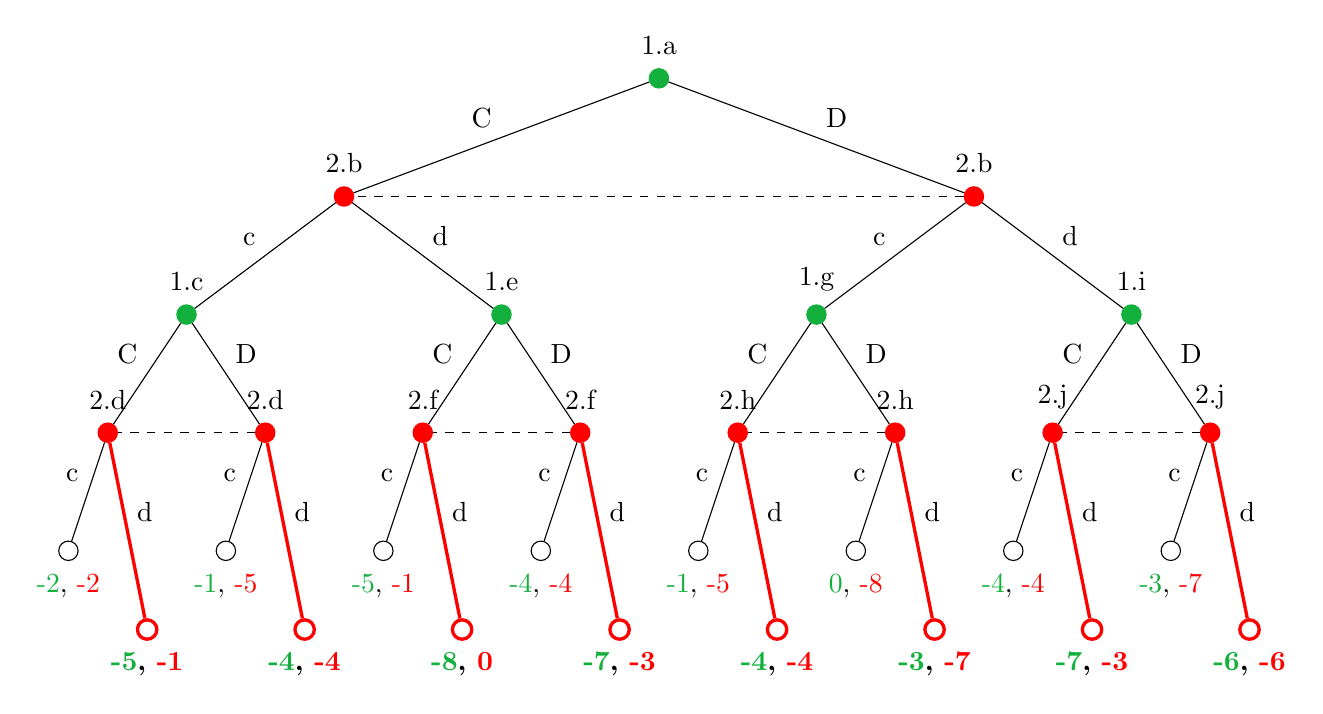
\begin{tikzpicture}
\node[noeud-std, color=green] (n1) {}
   [sibling distance=8cm]
      child {node[noeud-std, color=red] (n2-1c) {} % 1
      [sibling distance=4cm]
             child{node[noeud-std, color=green] (n1-1c2c){} % 2
                [sibling distance=2cm]
                child{node[noeud-std, color=red] (n2-1c2c1c){}  % 1
                    [sibling distance = 1cm]
                         child[level distance=1.5cm]{node[noeud-std,fill=white] (p-1c2c1c2c){} } % 1
                         child[level distance=2.5cm, very thick, red]{node[noeud-std,fill=white] (p-1c2c1c2d){} } % 1
                     }
                child{node[noeud-std, color=red] (n2-1c2c1d){}  % 1
                    [sibling distance = 1cm]
                        child[level distance=1.5cm]{node[noeud-std,fill=white] (p-1c2c1d2c){} } % 1
                        child[level distance=2.5cm, very thick, red]{node[noeud-std,fill=white] (p-1c2c1d2d){} } % 1
                    }
            }
            child{node[noeud-std, color=green] (n1-1c2d){} % 2
                [sibling distance=2cm]
                child{node[noeud-std, color=red] (n2-1c2d1c){}  % 1
                    [sibling distance = 1cm]
                         child[level distance=1.5cm]{node[noeud-std,fill=white] (p-1c2d1c2c){} } % 1
                         child[level distance=2.5cm, very thick, red]{node[noeud-std,fill=white] (p-1c2d1c2d){} } % 1
                     }
                child{node[noeud-std, color=red] (n2-1c2d1d){}  % 1
                    [sibling distance = 1cm]
                        child[level distance=1.5cm]{node[noeud-std,fill=white] (p-1c2d1d2c){} } % 1
                        child[level distance=2.5cm, very thick, red]{node[noeud-std,fill=white] (p-1c2d1d2d){} } % 1
                    }
            }
   }
   child {node[noeud-std, color=red] (n2-1d) {} % 1
      [sibling distance=4cm]
             child{node[noeud-std, color=green] (n1-1d2c){} % 2
                [sibling distance=2cm]
                child{node[noeud-std, color=red] (n2-1d2c1c){}  % 1
                    [sibling distance = 1cm]
                         child[level distance=1.5cm]{node[noeud-std,fill=white] (p-1d2c1c2c){} } % 1
                         child[level distance=2.5cm, very thick, red]{node[noeud-std,fill=white] (p-1d2c1c2d){} } % 1
                     }
                child{node[noeud-std, color=red] (n2-1d2c1d){}  % 1
                    [sibling distance = 1cm]
                        child[level distance=1.5cm]{node[noeud-std,fill=white] (p-1d2c1d2c){} } % 1
                        child[level distance=2.5cm, very thick, red]{node[noeud-std,fill=white] (p-1d2c1d2d){} } % 1
                    }
            }
            child{node[noeud-std, color=green] (n1-1d2d){} % 2
                [sibling distance=2cm]
                child{node[noeud-std, color=red] (n2-1d2d1c){}  % 1
                    [sibling distance = 1cm]
                         child[level distance=1.5cm]{node[noeud-std,fill=white] (p-1d2d1c2c){} } % 1
                         child[level distance=2.5cm, very thick, red]{node[noeud-std,fill=white] (p-1d2d1c2d){} } % 1
                     }
                child{node[noeud-std, color=red] (n2-1d2d1d){}  % 1
                    [sibling distance = 1cm]
                        child[level distance=1.5cm]{node[noeud-std,fill=white] (p-1d2d1d2c){} } % 1
                        child[level distance=2.5cm, very thick, red]{node[noeud-std,fill=white] (p-1d2d1d2d){} } % 1
                    }
            }
   }

;
%
\node[above=5pt] at (n1) {1.a};
\node[above left] at ($(n1)!{0.5}!(n2-1c)$) {C};
\node[above right] at ($(n1)!{0.5}!(n2-1d)$) {D};

\node[above=5pt] at (n2-1c) {2.b};
\node[above left] at ($(n2-1c)!{0.5}!(n1-1c2c)$) {c};
\node[above right] at ($(n2-1c)!{0.5}!(n1-1c2d)$) {d};
\node[above=5pt] at (n1-1c2c) {1.c};
\node[above left] at ($(n1-1c2c)!{0.5}!(n2-1c2c1c)$) {C};
\node[above right] at ($(n1-1c2c)!{0.5}!(n2-1c2c1d)$) {D};
\node[above=5pt] at (n2-1c2c1d) {2.d};
\node[above left] at ($(n2-1c2c1d)!{0.5}!(p-1c2c1d2c)$) {c};
\node[above right] at ($(n2-1c2c1d)!{0.5}!(p-1c2c1d2d)$) {d};
\node[above=5pt] at (n2-1c2c1c) {2.d};
\node[above left] at ($(n2-1c2c1c)!{0.5}!(p-1c2c1c2c)$) {c};
\node[above right] at ($(n2-1c2c1c)!{0.5}!(p-1c2c1c2d)$) {d};
\node[above=5pt] at (n1-1c2d) {1.e};
\node[above left] at ($(n1-1c2d)!{0.5}!(n2-1c2d1c)$) {C};
\node[above right] at ($(n1-1c2d)!{0.5}!(n2-1c2d1d)$) {D};
\node[above=5pt] at (n2-1c2d1d) {2.f};
\node[above left] at ($(n2-1c2d1d)!{0.5}!(p-1c2d1d2c)$) {c};
\node[above right] at ($(n2-1c2d1d)!{0.5}!(p-1c2d1d2d)$) {d};
\node[above=5pt] at (n2-1c2d1c) {2.f};
\node[above left] at ($(n2-1c2d1c)!{0.5}!(p-1c2d1c2c)$) {c};
\node[above right] at ($(n2-1c2d1c)!{0.5}!(p-1c2d1c2d)$) {d};

\node[above=5pt] at (n2-1d) {2.b};
\node[above left] at ($(n2-1d)!{0.5}!(n1-1d2c)$) {c};
\node[above right] at ($(n2-1d)!{0.5}!(n1-1d2d)$) {d};
\node[above=5pt] at (n1-1d2c) {1.g};
\node[above left] at ($(n1-1d2c)!{0.5}!(n2-1d2c1c)$) {C};
\node[above right] at ($(n1-1d2c)!{0.5}!(n2-1d2c1d)$) {D};
\node[above=5pt] at (n2-1d2c1d) {2.h};
\node[above left] at ($(n2-1d2c1d)!{0.5}!(p-1d2c1d2c)$) {c};
\node[above right] at ($(n2-1d2c1d)!{0.5}!(p-1d2c1d2d)$) {d};
\node[above=5pt] at (n2-1d2c1c) {2.h};
\node[above left] at ($(n2-1d2c1c)!{0.5}!(p-1d2c1c2c)$) {c};
\node[above right] at ($(n2-1d2c1c)!{0.5}!(p-1d2c1c2d)$) {d};
\node[above=5pt] at (n1-1d2d) {1.i};
\node[above left] at ($(n1-1d2d)!{0.5}!(n2-1d2d1c)$) {C};
\node[above right] at ($(n1-1d2d)!{0.5}!(n2-1d2d1d)$) {D};
\node[above=5pt] at (n2-1d2d1d) {2.j};
\node[above left] at ($(n2-1d2d1d)!{0.5}!(p-1d2d1d2c)$) {c};
\node[above right] at ($(n2-1d2d1d)!{0.5}!(p-1d2d1d2d)$) {d};
\node[above=5pt] at (n2-1d2d1c) {2.j};
\node[above left] at ($(n2-1d2d1c)!{0.5}!(p-1d2d1c2c)$) {c};
\node[above right] at ($(n2-1d2d1c)!{0.5}!(p-1d2d1c2d)$) {d};

\path (n2-1d)  edge [dashed] node {} (n2-1c);
\path (n2-1c2c1d)  edge [dashed] node {} (n2-1c2c1c);
\path (n2-1c2d1d)  edge [dashed] node {} (n2-1c2d1c);
\path (n2-1d2c1d)  edge [dashed] node {} (n2-1d2c1c);
\path (n2-1d2d1d)  edge [dashed] node {} (n2-1d2d1c);

\node[below = 5pt] at ($(p-1c2c1c2c)$) {\payoff{-2}{-2}};
\node[below = 5pt] at ($(p-1c2c1c2d)$) {\textbf{\payoff{-5}{-1}}};
\node[below = 5pt] at ($(p-1c2c1d2c)$) {\payoff{-1}{-5}};
\node[below = 5pt] at ($(p-1c2c1d2d)$) {\textbf{\payoff{-4}{-4}}};


\node[below = 5pt] at ($(p-1c2d1c2c)$) {\payoff{-5}{-1}};
\node[below = 5pt] at ($(p-1c2d1c2d)$) {\textbf{\payoff{-8}{0}}};
\node[below = 5pt] at ($(p-1c2d1d2c)$) {\payoff{-4}{-4}};
\node[below = 5pt] at ($(p-1c2d1d2d)$) {\textbf{\payoff{-7}{-3}}};


\node[below = 5pt] at ($(p-1d2c1c2c)$) {\payoff{-1}{-5}};
\node[below = 5pt] at ($(p-1d2c1c2d)$) {\textbf{\payoff{-4}{-4}}};
\node[below = 5pt] at ($(p-1d2c1d2c)$) {\payoff{0}{-8}};
\node[below = 5pt] at ($(p-1d2c1d2d)$) {\textbf{\payoff{-3}{-7}}};


\node[below = 5pt] at ($(p-1d2d1c2c)$) {\payoff{-4}{-4}};
\node[below = 5pt] at ($(p-1d2d1c2d)$) {\textbf{\payoff{-7}{-3}}};
\node[below = 5pt] at ($(p-1d2d1d2c)$) {\payoff{-3}{-7}};
\node[below = 5pt] at ($(p-1d2d1d2d)$) {\textbf{\payoff{-6}{-6}}};

\end{tikzpicture}}
\caption{Repeated Prisoner's Dilemma: backward induction step 1.}
\end{figure}

\end{frame}

\begin{frame}{Nash equilibrium: backward induction (2)}
    \begin{figure}[!ht]
    \centering
    \scalebox{0.65}{
    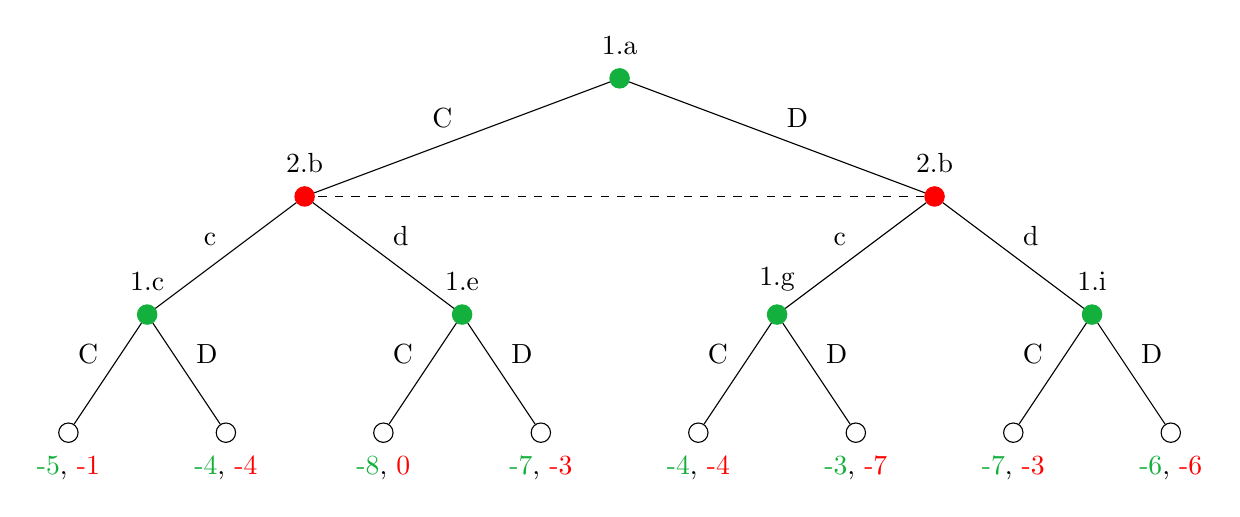
\begin{tikzpicture}
        \node[noeud-std, color=green] (n1) {}
           [sibling distance=8cm]
              child {node[noeud-std, color=red] (n2-1c) {} % 1
              [sibling distance=4cm]
                     child{node[noeud-std, color=green] (n1-1c2c){} % 2
                        [sibling distance=2cm]
                        child{node[noeud-std, fill=white] (n2-1c2c1c){}}
                        child{node[noeud-std, fill=white] (n2-1c2c1d){}}
                    }
                    child{node[noeud-std, color=green] (n1-1c2d){} % 2
                        [sibling distance=2cm]
                        child{node[noeud-std, fill=white] (n2-1c2d1c){}}
                        child{node[noeud-std, fill=white] (n2-1c2d1d){}}
                    }
           }
           child {node[noeud-std, color=red] (n2-1d) {} % 1
              [sibling distance=4cm]
                     child{node[noeud-std, color=green] (n1-1d2c){} % 2
                        [sibling distance=2cm]
                        child{node[noeud-std, fill=white] (n2-1d2c1c){}}
                        child{node[noeud-std, fill=white] (n2-1d2c1d){}}
                    }
                    child{node[noeud-std, color=green] (n1-1d2d){} % 2
                        [sibling distance=2cm]
                        child{node[noeud-std, fill=white] (n2-1d2d1c){}}
                        child{node[noeud-std, fill=white] (n2-1d2d1d){}}
                    }
           }
        ;
        %
        \node[above=5pt] at (n1) {1.a};
        \node[above left] at ($(n1)!{0.5}!(n2-1c)$) {C};
        \node[above right] at ($(n1)!{0.5}!(n2-1d)$) {D};

        \node[above=5pt] at (n2-1c) {2.b};
        \node[above left] at ($(n2-1c)!{0.5}!(n1-1c2c)$) {c};
        \node[above right] at ($(n2-1c)!{0.5}!(n1-1c2d)$) {d};
        \node[above=5pt] at (n1-1c2c) {1.c};
        \node[above left] at ($(n1-1c2c)!{0.5}!(n2-1c2c1c)$) {C};
        \node[above right] at ($(n1-1c2c)!{0.5}!(n2-1c2c1d)$) {D};
        \node[above=5pt] at (n1-1c2d) {1.e};
        \node[above left] at ($(n1-1c2d)!{0.5}!(n2-1c2d1c)$) {C};
        \node[above right] at ($(n1-1c2d)!{0.5}!(n2-1c2d1d)$) {D};

        \node[above=5pt] at (n2-1d) {2.b};
        \node[above left] at ($(n2-1d)!{0.5}!(n1-1d2c)$) {c};
        \node[above right] at ($(n2-1d)!{0.5}!(n1-1d2d)$) {d};
        \node[above=5pt] at (n1-1d2c) {1.g};
        \node[above left] at ($(n1-1d2c)!{0.5}!(n2-1d2c1c)$) {C};
        \node[above right] at ($(n1-1d2c)!{0.5}!(n2-1d2c1d)$) {D};
        \node[above=5pt] at (n1-1d2d) {1.i};
        \node[above left] at ($(n1-1d2d)!{0.5}!(n2-1d2d1c)$) {C};
        \node[above right] at ($(n1-1d2d)!{0.5}!(n2-1d2d1d)$) {D};

        \path (n2-1d)  edge [dashed] node {} (n2-1c);

        \node[below = 5pt] at ($(n2-1c2c1c)$) {\payoff{-5}{-1}};
        \node[below = 5pt] at ($(n2-1c2c1d)$) {\payoff{-4}{-4}};

        \node[below = 5pt] at ($(n2-1c2d1c)$) {\payoff{-8}{0}};
        \node[below = 5pt] at ($(n2-1c2d1d)$) {\payoff{-7}{-3}};

        \node[below = 5pt] at ($(n2-1d2c1c)$) {\payoff{-4}{-4}};
        \node[below = 5pt] at ($(n2-1d2c1d)$) {\payoff{-3}{-7}};

        \node[below = 5pt] at ($(n2-1d2d1c)$) {\payoff{-7}{-3}};
        \node[below = 5pt] at ($(n2-1d2d1d)$) {\payoff{-6}{-6}};
    \end{tikzpicture}}
    \caption{Repeated Prisoner's Dilemma: backward induction step 2.}
    \end{figure}
\end{frame}

\begin{frame}{Nash equilibrium: backward induction (3)}
    \begin{figure}[!ht]
    \centering
    \scalebox{0.65}{
    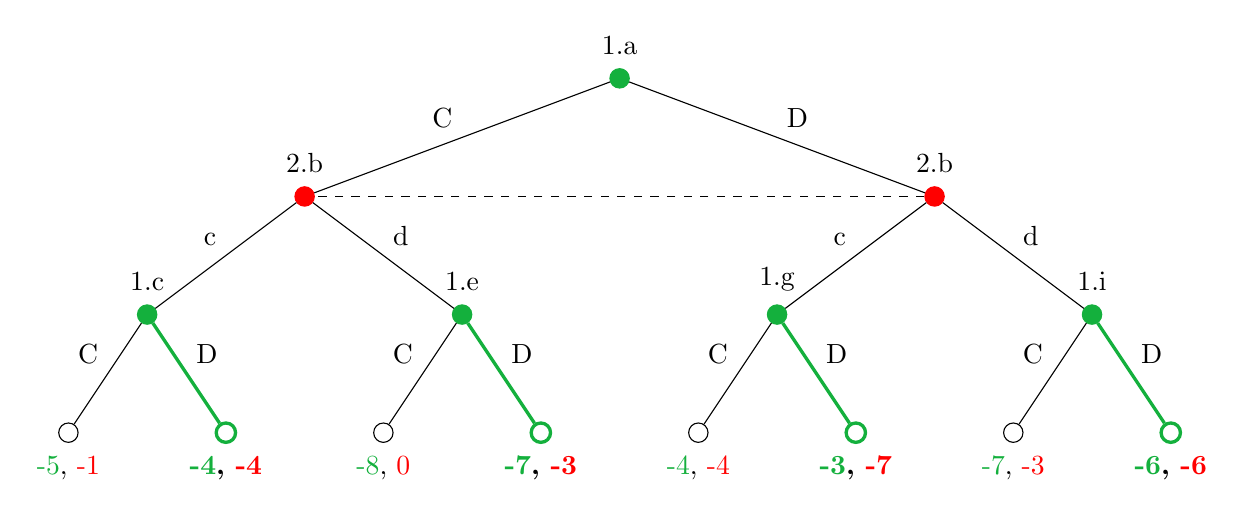
\begin{tikzpicture}
        \node[noeud-std, color=green] (n1) {}
           [sibling distance=8cm]
              child {node[noeud-std, color=red] (n2-1c) {} % 1
              [sibling distance=4cm]
                     child{node[noeud-std, color=green] (n1-1c2c){} % 2
                        [sibling distance=2cm]
                        child{node[noeud-std, fill=white] (n2-1c2c1c){}}
                        child[very thick, green]{node[noeud-std, fill=white] (n2-1c2c1d){}}
                    }
                    child{node[noeud-std, color=green] (n1-1c2d){} % 2
                        [sibling distance=2cm]
                        child{node[noeud-std, fill=white] (n2-1c2d1c){}}
                        child[very thick, green]{node[noeud-std, fill=white] (n2-1c2d1d){}}
                    }
           }
           child {node[noeud-std, color=red] (n2-1d) {} % 1
              [sibling distance=4cm]
                     child{node[noeud-std, color=green] (n1-1d2c){} % 2
                        [sibling distance=2cm]
                        child{node[noeud-std, fill=white] (n2-1d2c1c){}}
                        child[very thick, green]{node[noeud-std, fill=white] (n2-1d2c1d){}}
                    }
                    child{node[noeud-std, color=green] (n1-1d2d){} % 2
                        [sibling distance=2cm]
                        child{node[noeud-std, fill=white] (n2-1d2d1c){}}
                        child[very thick, green]{node[noeud-std, fill=white] (n2-1d2d1d){}}
                    }
           }
        ;
        %
        \node[above=5pt] at (n1) {1.a};
        \node[above left] at ($(n1)!{0.5}!(n2-1c)$) {C};
        \node[above right] at ($(n1)!{0.5}!(n2-1d)$) {D};

        \node[above=5pt] at (n2-1c) {2.b};
        \node[above left] at ($(n2-1c)!{0.5}!(n1-1c2c)$) {c};
        \node[above right] at ($(n2-1c)!{0.5}!(n1-1c2d)$) {d};
        \node[above=5pt] at (n1-1c2c) {1.c};
        \node[above left] at ($(n1-1c2c)!{0.5}!(n2-1c2c1c)$) {C};
        \node[above right] at ($(n1-1c2c)!{0.5}!(n2-1c2c1d)$) {D};
        \node[above=5pt] at (n1-1c2d) {1.e};
        \node[above left] at ($(n1-1c2d)!{0.5}!(n2-1c2d1c)$) {C};
        \node[above right] at ($(n1-1c2d)!{0.5}!(n2-1c2d1d)$) {D};

        \node[above=5pt] at (n2-1d) {2.b};
        \node[above left] at ($(n2-1d)!{0.5}!(n1-1d2c)$) {c};
        \node[above right] at ($(n2-1d)!{0.5}!(n1-1d2d)$) {d};
        \node[above=5pt] at (n1-1d2c) {1.g};
        \node[above left] at ($(n1-1d2c)!{0.5}!(n2-1d2c1c)$) {C};
        \node[above right] at ($(n1-1d2c)!{0.5}!(n2-1d2c1d)$) {D};
        \node[above=5pt] at (n1-1d2d) {1.i};
        \node[above left] at ($(n1-1d2d)!{0.5}!(n2-1d2d1c)$) {C};
        \node[above right] at ($(n1-1d2d)!{0.5}!(n2-1d2d1d)$) {D};

        \path (n2-1d)  edge [dashed] node {} (n2-1c);

        \node[below = 5pt] at ($(n2-1c2c1c)$) {\payoff{-5}{-1}};
        \node[below = 5pt] at ($(n2-1c2c1d)$) {\textbf{\payoff{-4}{-4}}};

        \node[below = 5pt] at ($(n2-1c2d1c)$) {\payoff{-8}{0}};
        \node[below = 5pt] at ($(n2-1c2d1d)$) {\textbf{\payoff{-7}{-3}}};

        \node[below = 5pt] at ($(n2-1d2c1c)$) {\payoff{-4}{-4}};
        \node[below = 5pt] at ($(n2-1d2c1d)$) {\textbf{\payoff{-3}{-7}}};

        \node[below = 5pt] at ($(n2-1d2d1c)$) {\payoff{-7}{-3}};
        \node[below = 5pt] at ($(n2-1d2d1d)$) {\textbf{\payoff{-6}{-6}}};
    \end{tikzpicture}}
    \caption{Repeated Prisoner's Dilemma: backward induction step 3.}
    \end{figure}
\end{frame}

\begin{frame}{Nash equilibrium: backward induction (4)}
    \begin{figure}[!ht]
        \centering
        \scalebox{0.65}{
        \begin{tikzpicture}
            \node[noeud-std, color=green] (n1) {}
               [sibling distance=8cm]
                  child {node[noeud-std, color=red] (n2-1c) {} % 1
                  [sibling distance=4cm]
                        child{node[noeud-std, fill=white] (n1-1c2c){}}
                        child{node[noeud-std, fill=white] (n1-1c2d){}}
               }
               child {node[noeud-std, color=red] (n2-1d) {} % 1
                  [sibling distance=4cm]
                        child{node[noeud-std, fill=white] (n1-1d2c){}}
                        child{node[noeud-std, fill=white] (n1-1d2d){}}
               }
            ;
            %
            \node[above=5pt] at (n1) {1.a};
            \node[above left] at ($(n1)!{0.5}!(n2-1c)$) {C};
            \node[above right] at ($(n1)!{0.5}!(n2-1d)$) {D};

            \node[above=5pt] at (n2-1c) {2.b};
            \node[above left] at ($(n2-1c)!{0.5}!(n1-1c2c)$) {c};
            \node[above right] at ($(n2-1c)!{0.5}!(n1-1c2d)$) {d};

            \node[above=5pt] at (n2-1d) {2.b};
            \node[above left] at ($(n2-1d)!{0.5}!(n1-1d2c)$) {c};
            \node[above right] at ($(n2-1d)!{0.5}!(n1-1d2d)$) {d};

            \path (n2-1d)  edge [dashed] node {} (n2-1c);

            \node[below = 5pt] at ($(n1-1c2c)$) {\payoff{-4}{-4}};
            \node[below = 5pt] at ($(n1-1c2d)$) {\payoff{-7}{-3}};
            \node[below = 5pt] at ($(n1-1d2c)$) {\payoff{-3}{-7}};
            \node[below = 5pt] at ($(n1-1d2d)$) {\payoff{-6}{-6}};
        \end{tikzpicture}}
        \caption{Repeated Prisoner's Dilemma: backward induction step 4.}
    \end{figure}
\end{frame}

\begin{frame}{Nash equilibrium: backward induction (5)}
    \begin{figure}[!ht]
        \centering
        \scalebox{0.65}{
        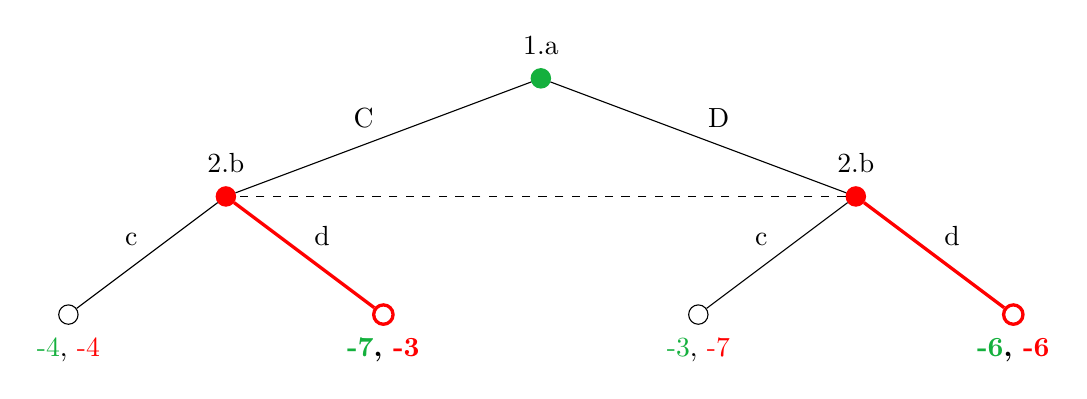
\begin{tikzpicture}
            \node[noeud-std, color=green] (n1) {}
               [sibling distance=8cm]
                  child {node[noeud-std, color=red] (n2-1c) {} % 1
                  [sibling distance=4cm]
                        child{node[noeud-std, fill=white] (n1-1c2c){}}
                        child[very thick, red]{node[noeud-std, fill=white] (n1-1c2d){}}
               }
               child {node[noeud-std, color=red] (n2-1d) {} % 1
                  [sibling distance=4cm]
                        child{node[noeud-std, fill=white] (n1-1d2c){}}
                        child[very thick, red]{node[noeud-std, fill=white] (n1-1d2d){}}
               }
            ;
            %
            \node[above=5pt] at (n1) {1.a};
            \node[above left] at ($(n1)!{0.5}!(n2-1c)$) {C};
            \node[above right] at ($(n1)!{0.5}!(n2-1d)$) {D};

            \node[above=5pt] at (n2-1c) {2.b};
            \node[above left] at ($(n2-1c)!{0.5}!(n1-1c2c)$) {c};
            \node[above right] at ($(n2-1c)!{0.5}!(n1-1c2d)$) {d};

            \node[above=5pt] at (n2-1d) {2.b};
            \node[above left] at ($(n2-1d)!{0.5}!(n1-1d2c)$) {c};
            \node[above right] at ($(n2-1d)!{0.5}!(n1-1d2d)$) {d};

            \path (n2-1d)  edge [dashed] node {} (n2-1c);

            \node[below = 5pt] at ($(n1-1c2c)$) {\payoff{-4}{-4}};
            \node[below = 5pt] at ($(n1-1c2d)$) {\textbf{\payoff{-7}{-3}}};
            \node[below = 5pt] at ($(n1-1d2c)$) {\payoff{-3}{-7}};
            \node[below = 5pt] at ($(n1-1d2d)$) {\textbf{\payoff{-6}{-6}}};
        \end{tikzpicture}}
        \caption{Repeated Prisoner's Dilemma: backward induction step 5.}
    \end{figure}
\end{frame}

\begin{frame}{Nash equilibrium: backward induction (6)}
    \begin{figure}[!ht]
        \centering
        \scalebox{0.65}{
        \begin{tikzpicture}
            \node[noeud-std, color=green] (n1) {}
                [sibling distance=8cm]
                    child {node[noeud-std, fill=white] (n2-1c) {}}
                    child {node[noeud-std, fill=white] (n2-1d) {} }
            ;
            %
            \node[above=5pt] at (n1) {1.a};
            \node[above left] at ($(n1)!{0.5}!(n2-1c)$) {C};
            \node[above right] at ($(n1)!{0.5}!(n2-1d)$) {D};

            \node[below = 5pt] at ($(n2-1c)$) {\payoff{-7}{-3}};
            \node[below = 5pt] at ($(n2-1d)$) {\payoff{-6}{-6}};
        \end{tikzpicture}}
        \caption{Repeated Prisoner's Dilemma: backward induction step 6.}
    \end{figure}
\end{frame}

\begin{frame}{Nash equilibrium: backward induction (7)}
    \begin{figure}[!ht]
        \centering
        \scalebox{0.65}{
        \begin{tikzpicture}
            \node[noeud-std, color=green] (n1) {}
                [sibling distance=8cm]
                    child {node[noeud-std, fill=white] (n2-1c) {}}
                    child[very thick, green] {node[noeud-std, fill=white] (n2-1d) {} }
            ;
            %
            \node[above=5pt] at (n1) {1.a};
            \node[above left] at ($(n1)!{0.5}!(n2-1c)$) {C};
            \node[above right] at ($(n1)!{0.5}!(n2-1d)$) {D};

            \node[below = 5pt] at ($(n2-1c)$) {\payoff{-7}{-3}};
            \node[below = 5pt] at ($(n2-1d)$) {\textbf{\payoff{-6}{-6}}};
        \end{tikzpicture}}
        \caption{Repeated Prisoner's Dilemma: backward induction step 7.}
    \end{figure}

    \begin{block}{Conclusion}
        The only Nash Equilibrium is for both players to defect at each round, leading
        to the total payoff (\payoff{-6}{-6}).
    \end{block}
\end{frame}

\note{
    Some people might argue at this point (or after the next slide) that we could implement
    a strategy with a punishment system to refrain the other player to defect. However, this
    threat of punishment is not subgame-perfect (i.e. not credible).
}

\begin{frame}{Take-home message \#1}
    \metroset{block=fill}
    \begin{block}{Take-home message \#1}
        Repeating the same game $K$ times where $K$ is known by the players before the game starts
        \textbf{do not} change the Nash equilibrium.\\\
        
        Proof? Use backward induction.
    \end{block}

    \textbf{Does this prediction match actual human behaviors?}
    No, see the following paper (and references inside).\\
    \fullcite{pd-repeated-real-life}.
\end{frame}

\begin{frame}[standout]
    Questions?
\end{frame}

\end{document}
